%%%%%%%%%%%%%%%%%%%%%%%%%%%%%%%%%%%%%%%%%%%%
% 
% Last edits: December, 2016
%%%%%%%%%%%%%%%%%%%%%%%%%%%%%%%%%%%%%%%%%%%%

\documentclass[12pt]{article}
\usepackage{natbib}
\usepackage[letterpaper, margin=1.1in]{geometry}
\usepackage{graphicx}
\usepackage{wrapfig}
\usepackage{enumitem}
\setlist[enumerate]{itemsep=0mm}
\usepackage{multirow}
\usepackage[table,xcdraw]{xcolor}
\usepackage{lscape}
\usepackage{caption}
\usepackage{subcaption}
\usepackage{hyperref}
\usepackage{bm}
\usepackage{float}
\usepackage{amsmath}
\renewcommand{\vector}[1]{\mathbf{#1}}


\begin{document}
\noindent{Alexandra Pulwicki \\ \today}

\begin{center}
\Large \textbf{Results\\ Basin Scale}
\end{center}

\section*{Overview}
This is a document that shows the sampled and full ranges of topographic parameters and then goes into the multiple linear regression and Bayesian model averaging that was used to explain SWE with topographic parameters. 

\tableofcontents
\pagebreak

%%%%
\section{Topographic parameters of study sites}
%%%%

\subsection{Creating DEM}

Topographic parameters can be derived from a digital elevation model (DEM) of the study area. The DEM used in this project was created from imagery taken with the SPOT-5 satellite and it was provided at no cost by the French Space Agency (CNES) through the SPIRIT International Polar Year project \citep{Korona2009}. The DEM has a cell size of 40$\times$40 m. 

**Two DEMs were available for the Donjek Range. The first DEM (???) covered all three study glaciers but a large part of Glacier 4 and some areas of Glacier 2 were masked by clouds, resulting in incorrect elevation data. The second DEM spans only part of the Donjek Range, covering most of Glacier 4 and a large portion of Glacier 2. This DEM had no cloud cover over Glacier 2 and 4. As a result, it was decided to merge the two DEMs to create a cloud free DEM that spanned all three glaciers. 

The merging process was complicated by the fact that there was a discrepancy in elevation values between the two DEMs. The second DEM had generally higher elevation values by about 10 m. Although the discrepancy was not consistent throughout the study area, the second DEM was generally higher than the first. ...


\subsection{Calculating topographic parameters}

Topographic parameters are used to describe local topography that affects snow distribution and act as proxies for physical processes that determine snow deposition and redistribution. Topographic parameters used in snow accumulation studies on glaciers include elevation ($z$), distance from centreline ($d_C$), slope ($m$), tangential ($\kappa_T$) and profile ($\kappa_P$) curvature, ``northness'' ($N$), aspect ($\alpha$), and $Sx$, which is a proxy for wind redistribution \citep{Basist1994, Revuelto2014, McGrath2015}.	
 
A number of programs were used calculate topographic parameters from the SPOT-5 DEM. Distance from centreline and ``northness'' were calculated in Matlab. $Sx$ was determined using a executable obtained from Adam Winstral that follows the procedure outlined in \cite{Winstral2002}. The remaining parameters were calculated using the \texttt{r.slope.aspect} module in GRASS GIS software run through QGIS as defined in \cite{Mitavsova1993} and described in \cite{Hofierka2009}. 

The GRASS module implements a local polynomial approximation method of the form 
\begin{equation}
z(x,y) = a\cdot x^2 +b\cdot y^2 +c \cdot x\cdot y +d \cdot x + e\cdot y +f.
\end{equation}•
This polynomial is fitted to 9 grid points (3$\times$3 array) and the coefficients are determined by weighted least squares. 
First order partial derivatives are derived using Horn's formula \citep{Horn1981, Neteler2013} . The gradient can be expressed as
\begin{equation}
\nabla \bar{ \bm{z}} = \left( \frac{\partial z}{\partial x}, \frac{\partial z}{\partial y} \right) = \left( 2 \cdot a  \cdot x + c  \cdot y +d, 2 \cdot b  \cdot y + c  \cdot x + e \right) .
\end{equation}•
Since we are interested in the value of the centre cell ($x=y=0$), the gradient is simply 
\begin{equation}
\nabla \bar{ \bm{z}} = (f_x,f_y) = (d,e),
\end{equation}•
where $d$ and $e$ are given by
\begin{equation}
f_x = \frac{(z_7-z_9)+(2z_4-2z_6)+(z_1-z_3)}{8 \cdot \Delta x},\\
\end{equation}•
\begin{equation}
f_y = \frac{(z_7-z_1)+(2z_8-2z_2)+(z_9-z_3)}{8 \cdot \Delta y}.
\end{equation}•
Here, $z_k$ refers to one of the grid cells surrounding the cell of interest, which is located at row $i$ and column $j$ of the DEM. So $z_3 = z_{i+1,j+1}$, $z_7 = z_{i-1,j-1}$, and so on. $\Delta x$ and $\Delta y$ are the grid spacing (resolution) of the DEM. The second order partial derivatives can be written as \citep{Hofierka2009, Neteler2013}
\begin{align}
f_{xx} &= \frac{z_1-2z_2+z_3+4z_4-8z_5+4z_6+z_7-2z_8+z_9}{6 \cdot (\Delta x)^2},\\
f_{yy} &= \frac{z_1-4z_2+z_3-2z_4-8z_5-2z_6+z_7+4z_8+z_9}{6 \cdot (\Delta y)^2},\\
f_{xy} &= \frac{(z_7-z_9)-(z_1-z_3)}{4 \cdot \Delta x \Delta y}.
\end{align}
The second derivatives are most commonly used to calculate the curvature of a surface. The curvature at a given point on a curve is determined by finding the inverse of the radius of a circle that best fits the curve \citep{Olaya2009}. Convex surfaces have positive curvature and concave surfaces have negative curvature. 

The calculation of topographic parameters is described below.
\begin{enumerate}
\item[]\textbf{Elevation} values were taken from the SPOT-5 DEMs directly.

\item[] \textbf{Distance from centreline} was calculated as the minimum distance between the Easting and Northing of the northwest corner of each cell and a centreline that was drawn by hand in QGIS. This was completed in Matlab using the script `CentrelineDistance.m'. 

\item[]  \textbf{Slope} is taken to be the steepest slope angle and is the magnitude of gradient \citep{Mitavsova1993}. Using the gradient, it can be expressed as  \citep{Olaya2009}
	\begin{equation}
	m = \textrm{arctan}(|\nabla \bar{ \vector{z}}|) = \textrm{arctan} \left( \sqrt{(f_x)^2 +( f_y)^2} \right)
	\end{equation}•
\item[] \textbf{Tangential Curvature} (horizontal curvature) represents the curvature in the direction of the contour tangent. The equation for tangential curvature can be written as \citep{Olaya2009}
	\begin{equation}
	\kappa_T = - \frac{e^2 \cdot r -2 \cdot d\cdot e \cdot s +d^2 \cdot t}{(d^2+e^2) \cdot \sqrt{1+d^2+e^2}}
	\end{equation}•
where $d$ and $e$ are as above and
	\begin{align}
	r &= \frac{\partial^2 z}{\partial x^2} = \frac{z_1+z_3+z_4+z_6+z_7+z_9-2 \cdot (z_2+z_5+z_8)}{3 \cdot \Delta s^2}\\
	s &= \frac{\partial^2 z}{\partial x \partial y} = \frac{z_3 + z_7- z_1 - z_9}{4 \cdot \Delta s^2}\\
	t &= \frac{\partial^2 z}{\partial y^2} = \frac{z_1+z_2+z_3+z_7+z_8+z_9-2 \cdot (z_4+z_5+z_6)}{3 \cdot \Delta s^2}
	\end{align}•	

\item[] \textbf{Profile Curvature} (vertical curvature) represents the curvature in the direction of the the steepest slope (gradient). The equation for profile curvature can be written as \citep{Olaya2009}
	\begin{equation}
	\kappa_P = - \frac{d^2 \cdot r +2 \cdot d\cdot e \cdot r \cdot s +e^2 \cdot t}{(d^2+e^2) \cdot \sqrt{(1+d^2+e^2)^3}}
	\end{equation}•

\item[] \textbf{``Northness''} is defined as the product of the cosine of aspect and sine of slope \citep{Molotch2005}. A value of -1 represents a steep, south facing slope, a value of +1 represents a steep, north facing slope, and a flat surfaces yield 0. 

\item[] \textbf{Aspect} represent the orientation of the steepest slope, with 0${^\circ}$ defined as north and no value given to cells that have no gradient. Using the gradient, it can expressed as \citep{Olaya2009}
	\begin{equation}
	\alpha = 180 - \textrm{arctan}\left(\frac{ f_y}{ f_x}\right)+90 \cdot \frac{ f_x}{| f_x|}
	\end{equation}•

\item[] \textbf{\textit{Sx}} represents wind exposure/shelter and is based on selecting a cell within a certain angle and distance from the cell of interest that has the greatest upward slope relative to the cell of interest \citep{Winstral2002}. This can be referred to as the maximum upwind slope. Negative $Sx$ values represent exposure relative to the shelter-defining pixel, which means that the cell of interest was higher than the cell with greatest upward slope. Conversely, positive values represent sheltered cells. To determine $Sx$ values, we use the equation
\begin{equation}
Sx_{A, dmax}(x_i, y_i) = \textrm{max} \left[ \textrm{tan}^{-1} \left( \frac{z(x_v,y_v)-z(x_i,y_i)}{[(x_v-x_i)^2+(y_v-y_i)^2]^{1/2}} \right) \right] ,
\end{equation}
where A is the azimuth of the search direction, $(x_i, y_i)$ are the coordinates of the cell of interest, and $(x_v, y_v)$ are the set of all cell coordinates located along the search vector defined by	$(x_i, y_i)$, the azimuth ($A$), and maximum search distance ($d$max). Code for this calculation was provided by Adam Winstral (2016, personal communication). As done by \cite{McGrath2015}, we computed $Sx$ at 5$^{\circ}$ azimuth increments for $d$max distances of 100, 200, and 300 m. These values were then correlated with observed values of SWE and the azimuth and $d$max values with the highest correlation were used for subsequent analysis (see Table \ref{tab:Sxparams}). 

\begin{table}[]
\centering
\caption{Values of azimuth ($A$) and maximum search distance($d$max), which define the $Sx$ that had the highest correlation to observed SWE.}
\label{tab:Sxparams}
\begin{tabular}{lcc}
           & \textbf{$A$ ($^{\circ}$ from North)} & \textbf{\textit{d}max (m)} \\ \hline
Glacier 4  & 75                                & 200                 \\
Glacier 2  & 55                                & 200                 \\
Glacier 13 & 325                            & 200                
\end{tabular}
\end{table}

\end{enumerate}

\subsection{Topographic parameters from QGIS to Matlab}

The values of each topographic parameters at the sampling locations was determined in QGIS. The sampling locations were imported to QGIS and the Point Sampling Tool was used to determine the value of the cell of the raster for each topographic parameter at that location. This set of parameters that corresponded to each location was then exported to a .csv file and imported into Matlab with the script 'Import\_Topo.m'.  Note that selection of $Sx$ values was completed first (see above) and only the $Sx$ data with highest correlation to SWE was exported. After importing to Matlab, the sets of parameter values ($x_i$) were standardized ($x_s$) using the equation $x_s = \frac{x_i-\mu}{\sigma}$. The resulting structure is called \texttt{topo\_sampled} and is used in the MLR to be able to compare the explanatory power of each parameter (Section \ref{sec:MLR}). A non-standardized copy of the topographic parameters at the sampling locations was also kept for plotting purposes and is called is called \texttt{topo\_sampled\_ns}. Both structures are organized as a vector of values corresponding to the vectors in the \texttt{SWE} variable. 

The raster data for each topographic parameter was also exported from QGIS as a .csv file and then imported into Matlab with the script 'Import\_Topo.m'. The values are stored in the structure \texttt{topo\_full} and are a matrix, where each cell corresponds to one DEM cell. Cells outside of the glacier outline have no value (\texttt{NaN}).

\subsection{Parameter correlation}

The correlation between topographic parameters at sampling locations on each glacier is shown in Table \ref{tab:pearson_correlation}. Correlation values were generally low, with the exception of the correlation between northness and aspect on Glacier 4 and northness and elevation on Glacier 2, which were both negative and larger than 0.7. Since there is little correlation and correlation that varies between glaciers, the use of a multiple linear regression with these topographic parameters as predictor variables is warranted. 

\begin{table}[]
\centering
\caption{Pearson correlation coefficients between topographic parameters at sampled locations. The parameters include aspect ($\alpha$), elevation ($z$), northness ($N$), profile curvature ($\kappa_P$), slope ($m$), tangent curvature ($\kappa_T$), wind redistribution ($Sx$) and distance from centreline ($d_C$).}
\label{tab:pearson_correlation}
\begin{tabular}{cccccccccc}
\textbf{Glacier} &  & \textbf{$\alpha$} & \textbf{$z$} & \textbf{$N$} & \textbf{$\kappa_P$} & \textbf{$m$} & \textbf{$\kappa_T$} & \textbf{$Sx$} & \textbf{$d_C$} \\
\rowcolor[HTML]{EFEFEF} 
\cellcolor[HTML]{EFEFEF} & \textbf{$\alpha$} & 1 & 0.52 & -0.78 & 0.24 & -0.2 & 0.12 & 0.30 & -0.12 \\
\rowcolor[HTML]{EFEFEF} 
\cellcolor[HTML]{EFEFEF} & \textbf{$z$} & 0 & 1 & -0.53 & 0.16 & \textless 0.01 & 0.15 & 0.21 & 0.20 \\
\rowcolor[HTML]{EFEFEF} 
\cellcolor[HTML]{EFEFEF} & \textbf{$N$} & 0 & 0 & 1 & -0.33 & 0.07 & -0.13 & -0.49 & 0.09 \\
\rowcolor[HTML]{EFEFEF} 
\cellcolor[HTML]{EFEFEF} & \textbf{$\kappa_P$} & 0 & 0 & 0 & 1 & -0.20 & 0.44 & -0.30 & -0.16 \\
\rowcolor[HTML]{EFEFEF} 
\cellcolor[HTML]{EFEFEF} & \textbf{$m$} & 0 & 0 & 0 & 0 & 1 & \textless 0.01 & 0.20 & 0.36 \\
\rowcolor[HTML]{EFEFEF} 
\cellcolor[HTML]{EFEFEF} & \textbf{$\kappa_T$} & 0 & 0 & 0 & 0 & 0 & 1 & -0.28 & -0.01 \\
\rowcolor[HTML]{EFEFEF} 
\cellcolor[HTML]{EFEFEF} & \textbf{$Sx$} & 0 & 0 & 0 & 0 & 0 & 0 & 1 & 0.07 \\
\rowcolor[HTML]{EFEFEF} 
\multirow{-8}{*}{\cellcolor[HTML]{EFEFEF}Glacier 4} & \textbf{$d_C$} & 0 & 0 & 0 & 0 & 0 & 0 & 0 & 1 \\
 & \textbf{$\alpha$} & 1 & -0.02 & 0.04 & 0.13 & -0.16 & -0.02 & -0.02 & -0.12 \\
 & \textbf{$z$} & 0 & 1 & -0.62 & 0.06 & -0.46 & 0.02 & 0.14 & 0.05 \\
 & \textbf{$N$} & 0 & 0 & 1 & -0.03 & 0.5 & 0.09 & -0.15 & 0.32 \\
 & $\kappa_P$ & 0 & 0 & 0 & 1 & -0.01 & 0.45 & 0.01 & 0.08 \\
 & $m$ & 0 & 0 & 0 & 0 & 1 & -0.02 & -0.07 & 0.12 \\
 & $\kappa_T$ & 0 & 0 & 0 & 0 & 0 & 1 & -0.03 & 0.19 \\
 & $Sx$ & 0 & 0 & 0 & 0 & 0 & 0 & 1 & -0.18 \\
\multirow{-8}{*}{Glacier 2} & $d_C$ & 0 & 0 & 0 & 0 & 0 & 0 & 0 & 1 \\
\rowcolor[HTML]{EFEFEF} 
\cellcolor[HTML]{EFEFEF} & $\alpha$ & 1 & -0.24 & -0.07 & 0.02 & -0.1 & 0.02 & 0.08 & 0.06 \\
\rowcolor[HTML]{EFEFEF} 
\cellcolor[HTML]{EFEFEF} & $z$ & 0 & 1 & 0.14 & 0.08 & 0.01 & 0.01 & -0.24 & 0.13 \\
\rowcolor[HTML]{EFEFEF} 
\cellcolor[HTML]{EFEFEF} & $N$ & 0 & 0 & 1 & 0.06 & 0.24 & 0.08 & -0.01 & 0.07 \\
\rowcolor[HTML]{EFEFEF} 
\cellcolor[HTML]{EFEFEF} & $\kappa_P$ & 0 & 0 & 0 & 1 & -0.02 & 0.37 & -0.04 & 0.07 \\
\rowcolor[HTML]{EFEFEF} 
\cellcolor[HTML]{EFEFEF} & $m$ & 0 & 0 & 0 & 0 & 1 & -0.15 & -0.02 & 0.09 \\
\rowcolor[HTML]{EFEFEF} 
\cellcolor[HTML]{EFEFEF} & \textbf{$\kappa_T$} & 0 & 0 & 0 & 0 & 0 & 1 &\textless 0.01 & \textless 0.01 \\
\rowcolor[HTML]{EFEFEF} 
\cellcolor[HTML]{EFEFEF} & \textbf{$Sx$} & 0 & 0 & 0 & 0 & 0 & 0 & 1 & -0.06 \\
\rowcolor[HTML]{EFEFEF} 
\multirow{-8}{*}{\cellcolor[HTML]{EFEFEF}Glacier 13} & \textbf{$d_C$} & 0 & 0 & 0 & 0 & 0 & 0 & 0 & 1
\end{tabular}
\end{table}

\subsection{Maps of topographic parameters and range of parameters sampled}

\begin{landscape}

\begin{figure}
	\centering
	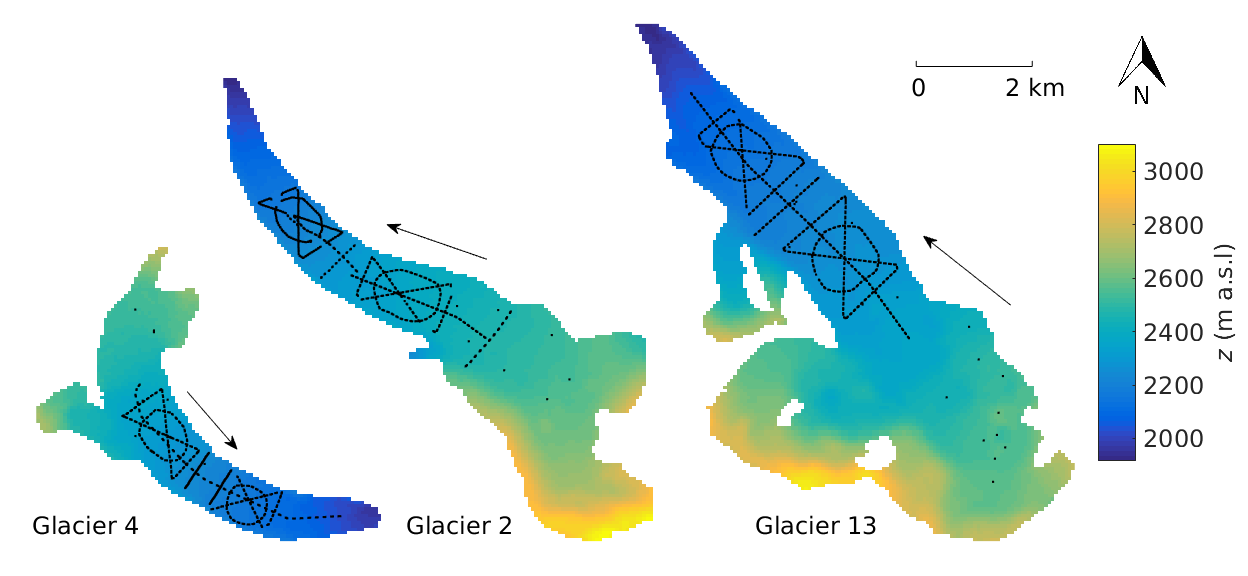
\includegraphics[height = 0.4\textwidth]{Map_elevation.png}\\
	\caption{Values of elevation used in the topographic regressions for three study glaciers. This DEM is derived from a SPOT5 satellite image and has a grid size of 40x40 m. Subsequent topographic parameters were derived from this DEM.}
	\label{map:elev}
\end{figure}

\begin{figure}
	\centering
	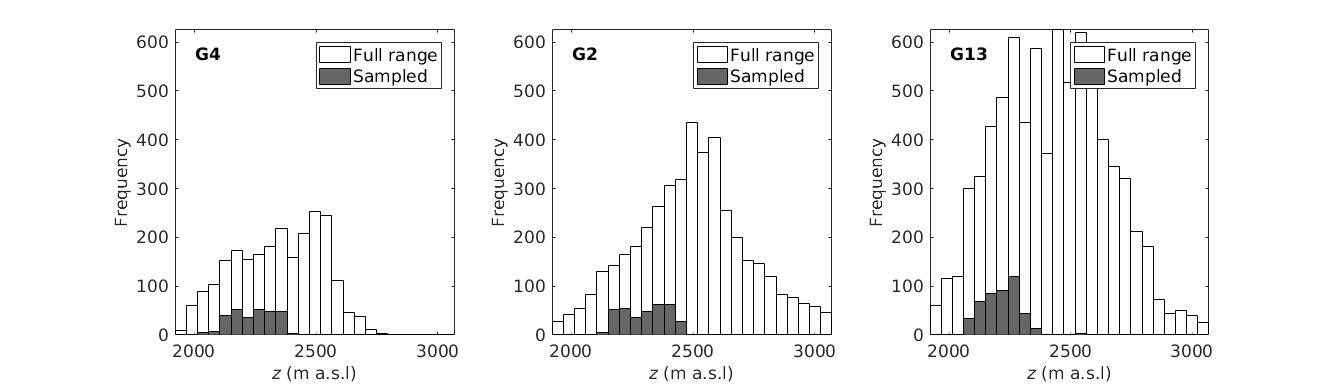
\includegraphics[height = 0.4\textwidth]{SampledRangeTopo_elevation.png}\\
	\caption{Range of elevation sampled as compared to total range of elevation of study glaciers.}
	\label{sampledRange:elev}
\end{figure}

\begin{figure}
	\centering
	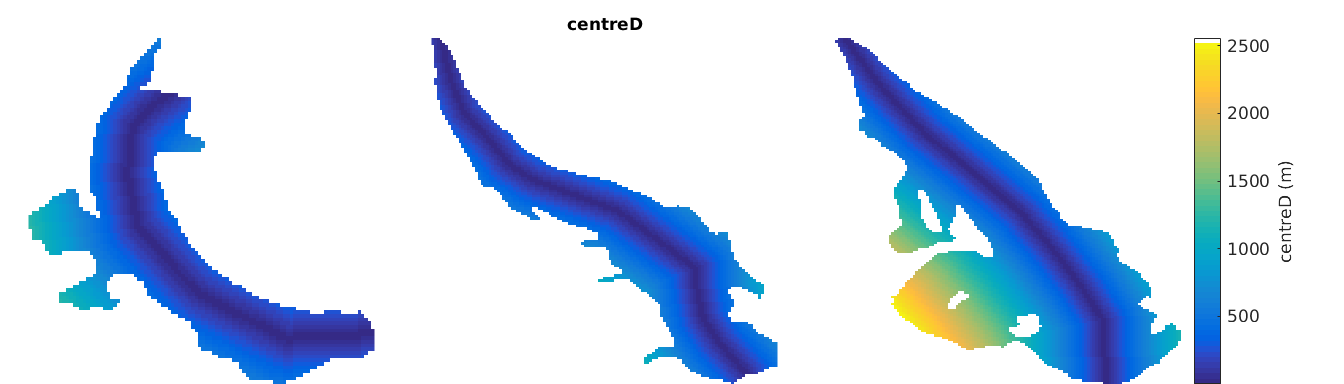
\includegraphics[height = 0.4\textwidth]{Map_centreD.png}\\
	\caption{Values of distance from centreline used in the topographic regressions for three study glaciers. Centreline was drawn by hand in QGIS.}
	\label{map:centreD}
\end{figure}

\begin{figure}
	\centering
	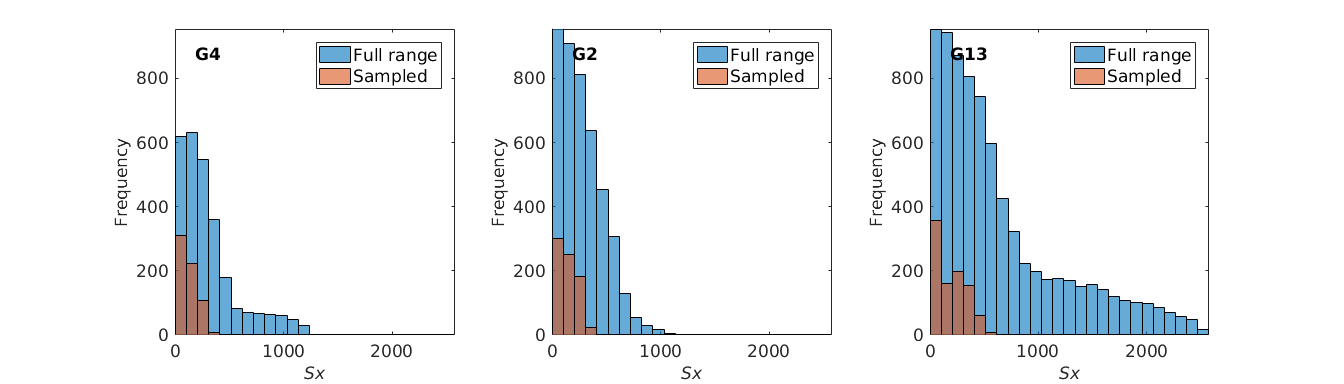
\includegraphics[height = 0.4\textwidth]{SampledRangeTopo_centreD.png}\\
	\caption{Range of distance from centreline sampled as compared to total range of distance from centreline of study glaciers.}
	\label{sampledRange:centreD}
\end{figure}

\begin{figure}
	\centering
	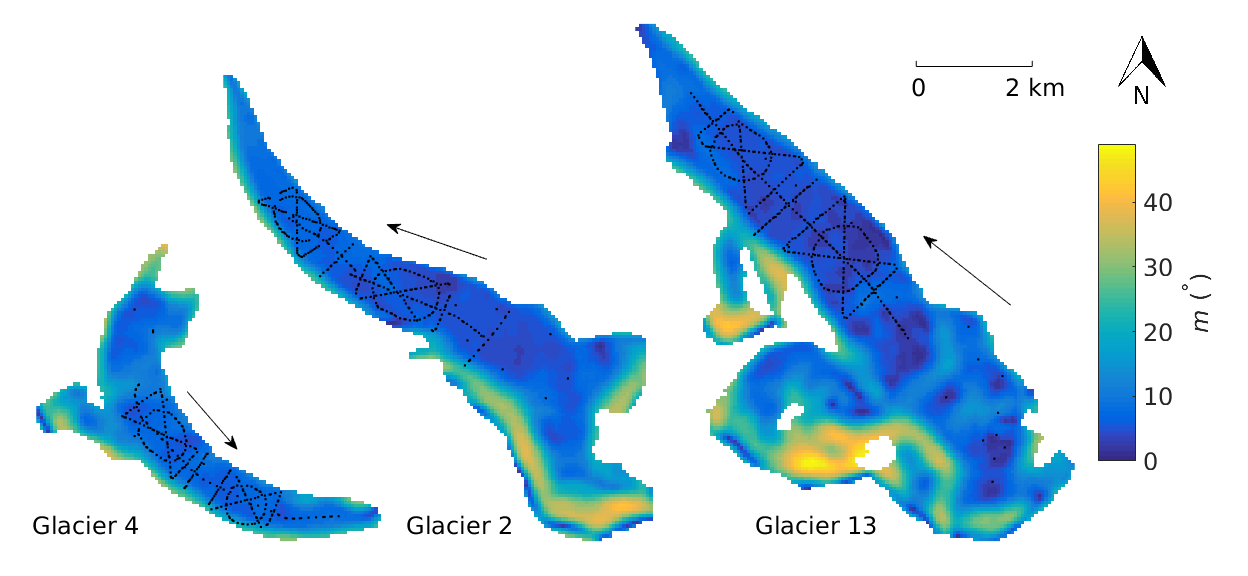
\includegraphics[height = 0.4\textwidth]{Map_slope.png}\\
	\caption{Values of slope used in the topographic regressions for three study glaciers. Values were derived from a SPOT5 satellite derived DEM (grid size of 40x40 m) in QGIS.}
	\label{map:slope}
\end{figure}

\begin{figure}
	\centering
	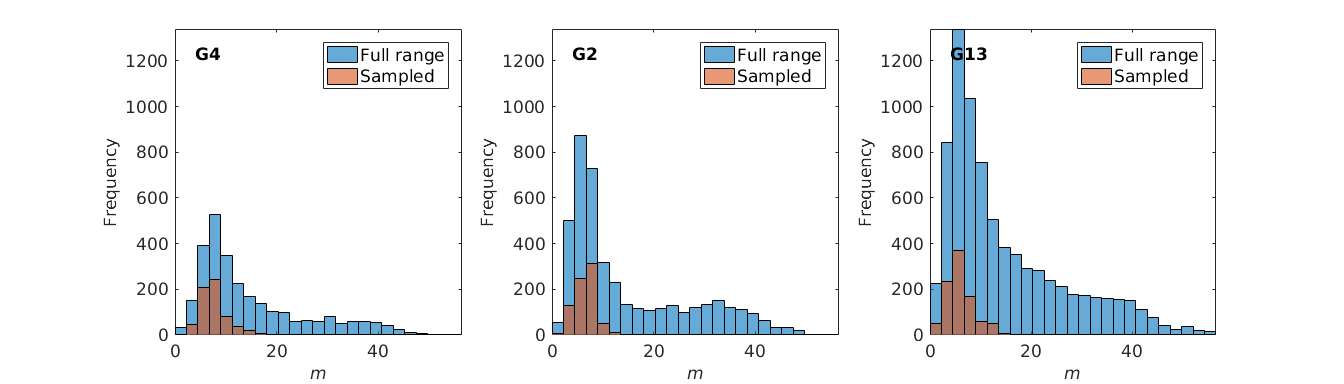
\includegraphics[height = 0.4\textwidth]{SampledRangeTopo_slope.png}\\
	\caption{Range of slope sampled as compared to total range of slope of study glaciers.}
	\label{sampledRange:slope}
\end{figure}

\begin{figure}
	\centering
	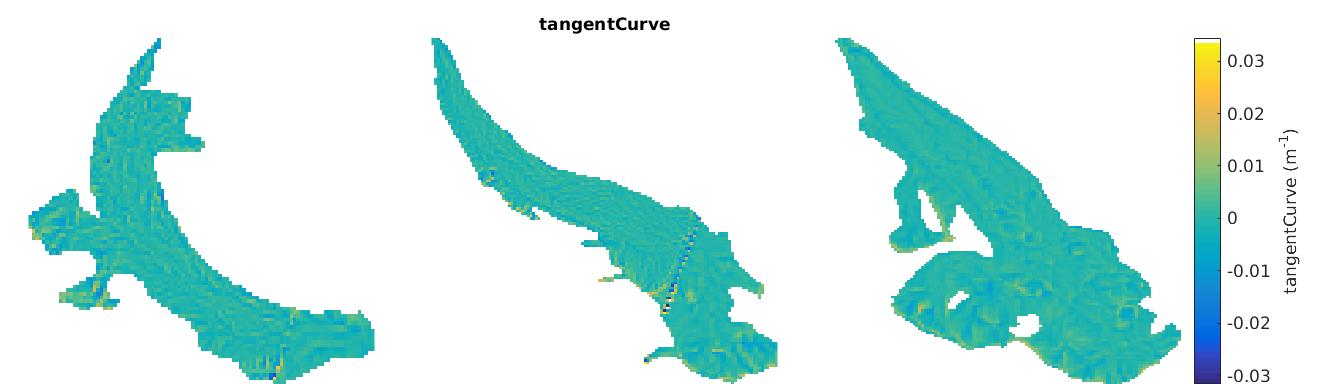
\includegraphics[height = 0.4\textwidth]{Map_tangentCurve.png}\\
	\caption{Values of tangential curvature used in the topographic regressions for three study glaciers. Values were derived from a SPOT5 satellite derived DEM (grid size of 40x40 m) in QGIS.}
	\label{map:tangentC}
\end{figure}

\begin{figure}
	\centering
	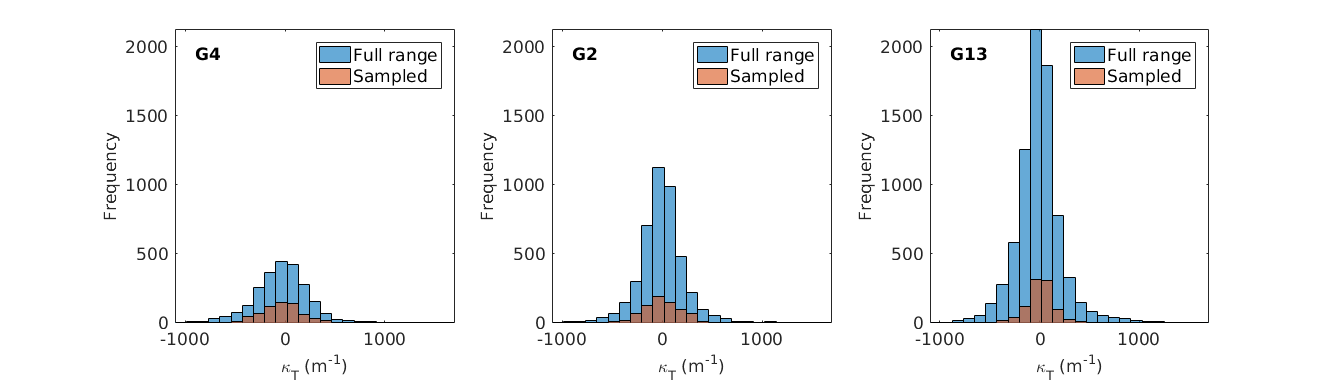
\includegraphics[height = 0.4\textwidth]{SampledRangeTopo_tangentCurve.png}\\
	\caption{Range of tangential curvature sampled as compared to total range of tangential curvature of study glaciers.}
	\label{sampledRange:tangentC}
\end{figure}

\begin{figure}
	\centering
	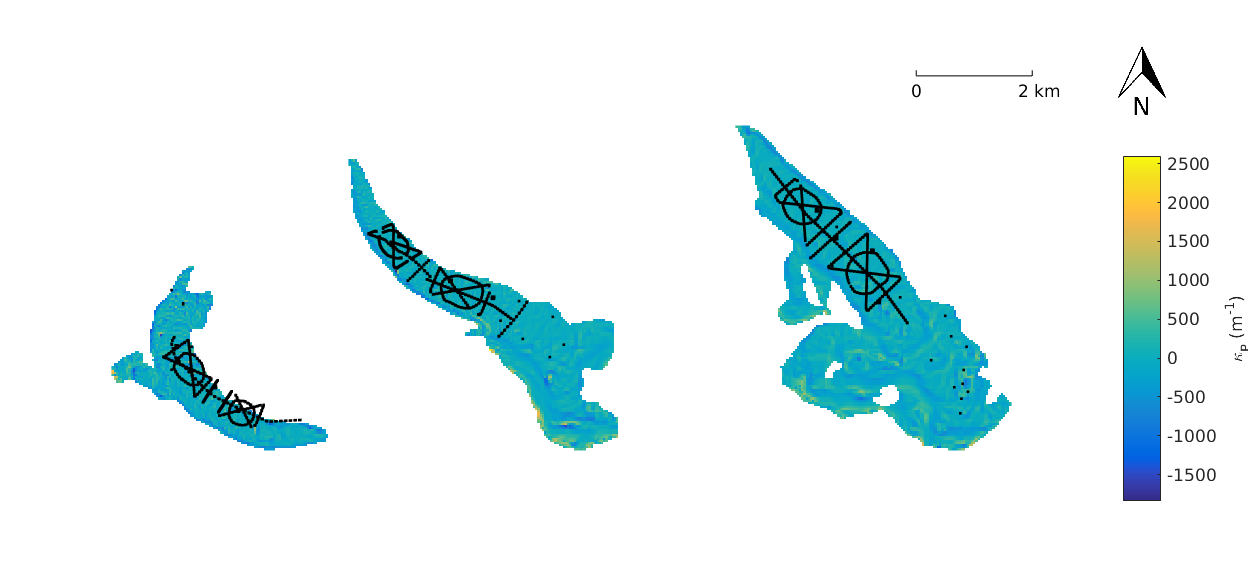
\includegraphics[height = 0.36\textwidth]{Map_profileCurve.png}\\
	\caption{Values of distance from centreline used in the topographic regressions for three study glaciers. Values were derived from a SPOT5 satellite derived DEM (grid size of 40x40 m) in QGIS.}
	\label{map:profileC}
\end{figure}

\begin{figure}
	\centering
	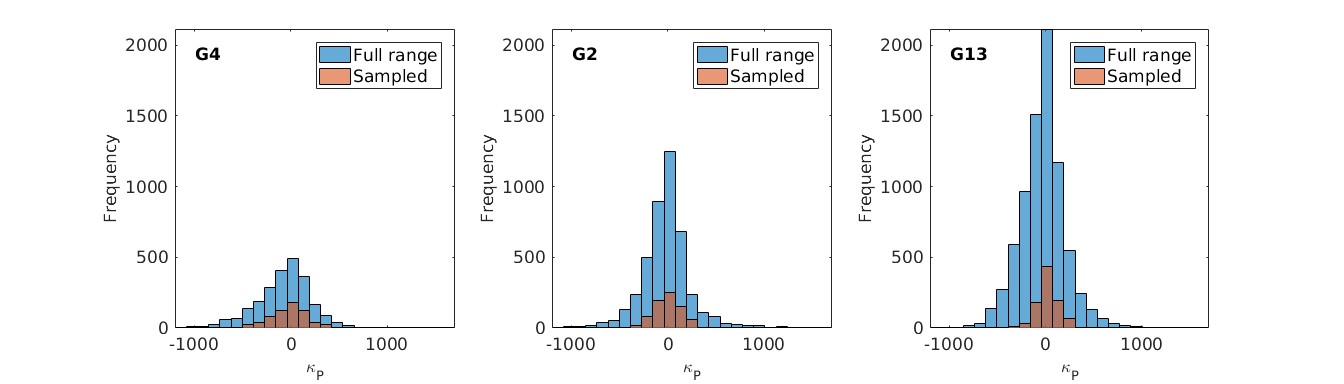
\includegraphics[height = 0.4\textwidth]{SampledRangeTopo_profileCurve.png}\\
	\caption{Range of profile curvature sampled as compared to total range of profile curvature of study glaciers.}
	\label{sampledRange:profileC}
\end{figure}


\begin{figure}
	\centering
	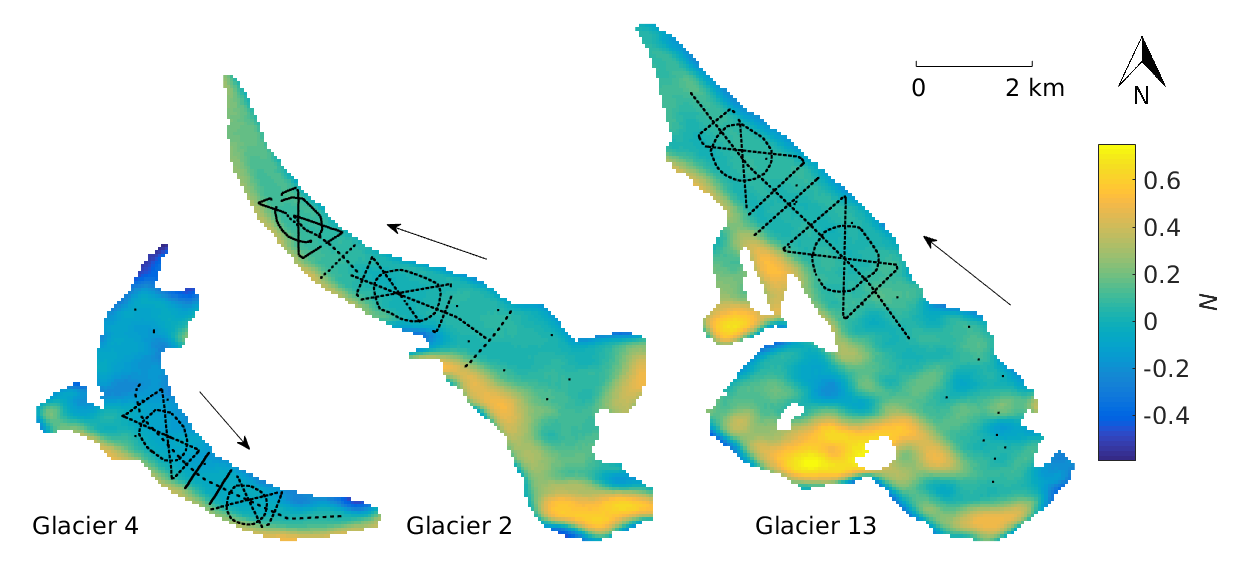
\includegraphics[height = 0.36\textwidth]{Map_northness.png}\\
	\caption{Values of ``northness'' used in the topographic regressions for three study glaciers. ``Northness'' is defined as the product of the cosine of aspect and sine of slope. A value of -1 represents a steep, south facing slope, a value of +1 represents a steep, north facing slope, and flat surfaces yield 0. Values were derived from a SPOT5 satellite derived DEM (grid size of 40x40 m) in QGIS.}
	\label{map:northness}
\end{figure}

\begin{figure}
	\centering
	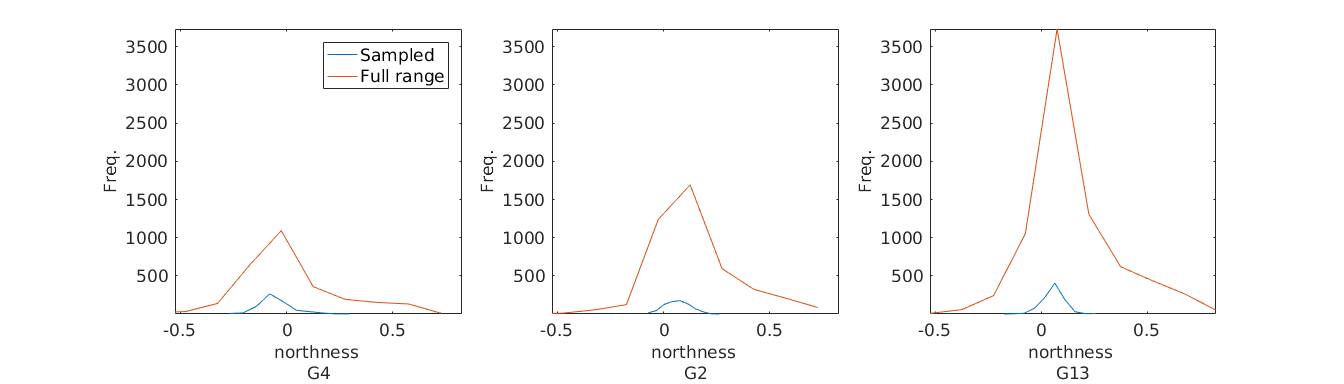
\includegraphics[height = 0.4\textwidth]{SampledRangeTopo_northness.png}\\
	\caption{Range of ``northness'' sampled as compared to total range of ``northness'' of study glaciers.}
	\label{sampledRange:northness}
\end{figure}

\begin{figure}
	\centering
	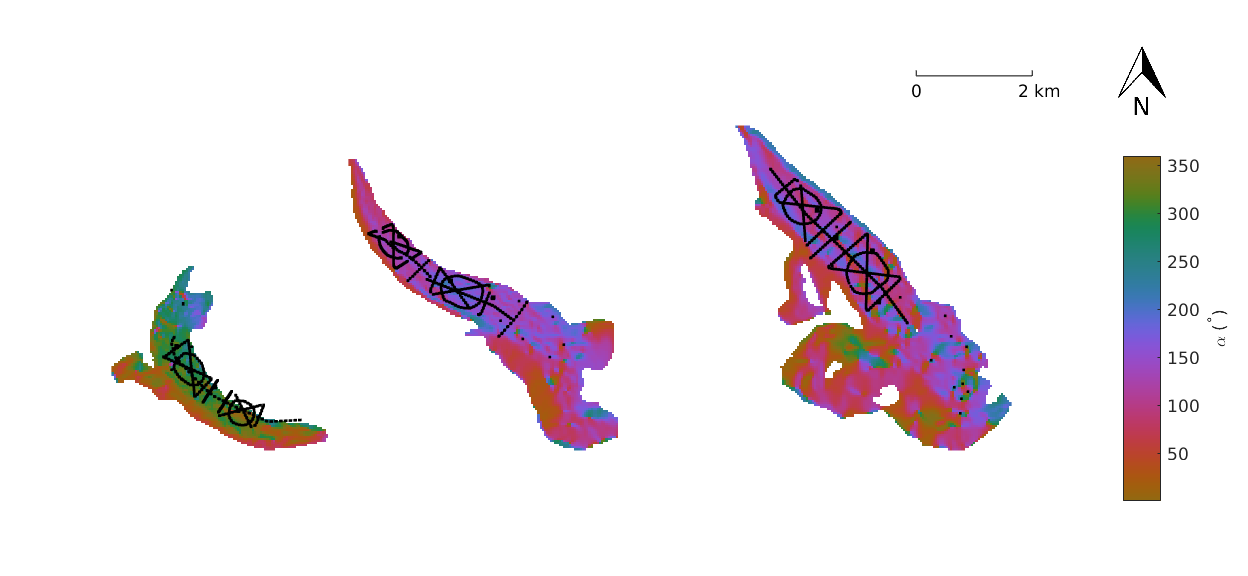
\includegraphics[height = 0.4\textwidth]{Map_aspect.png}\\
	\caption{Values of aspect, which represent what direction a slope is facing (0${^\circ}$ defined as north), used in the topographic regressions for three study glaciers.}
	\label{map:aspect}
\end{figure}

\begin{figure}
	\centering
	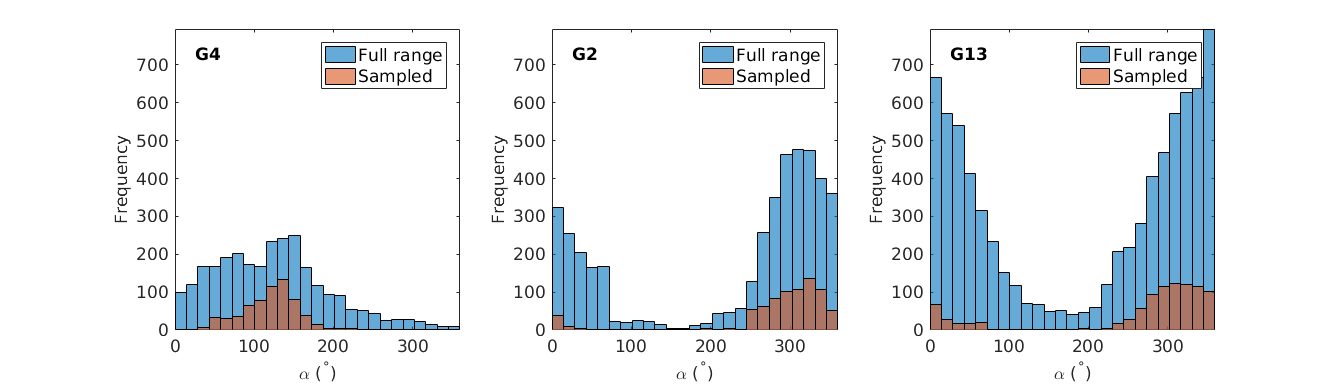
\includegraphics[height = 0.4\textwidth]{SampledRangeTopo_aspect.png}\\
	\caption{Range of aspect sampled as compared to total range of aspect of study glaciers.}
	\label{sampledRange:aspect}
\end{figure}

\begin{figure}
	\centering
	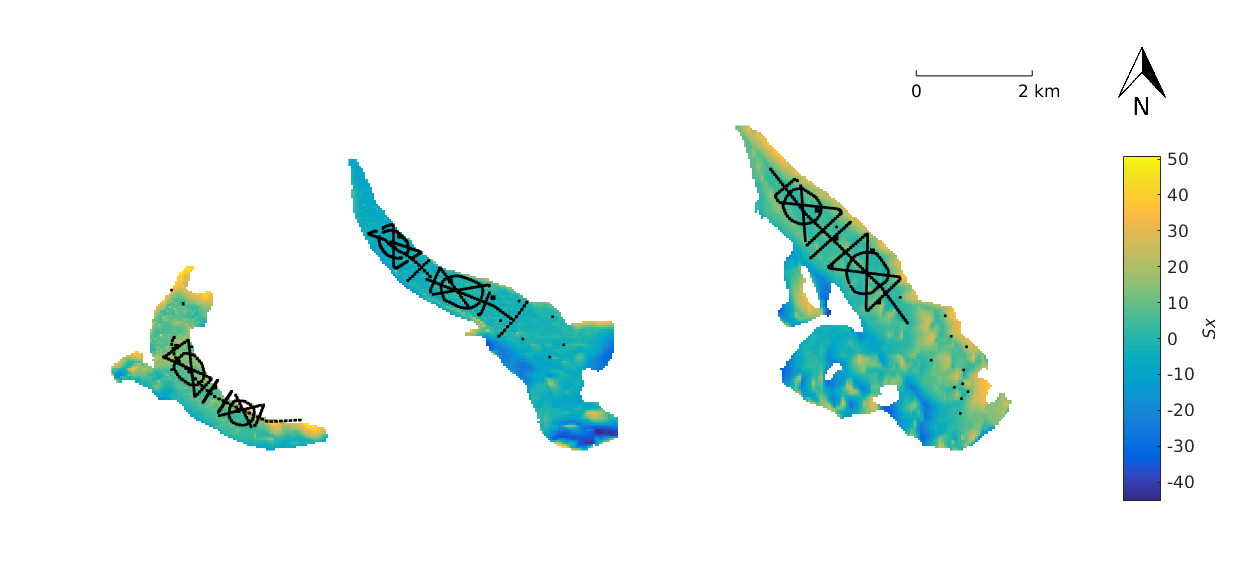
\includegraphics[height = 0.4\textwidth]{Map_Sx.png}\\
	\caption{Values of $Sx$, which is a wind redistribution parameter, used in the topographic regressions for three study glaciers. See section \ref{Sec:Sx} and the original paper by \cite{Winstral2002} for more details on calculation .}
	\label{map:Sx}
\end{figure}

\begin{figure}
	\centering
	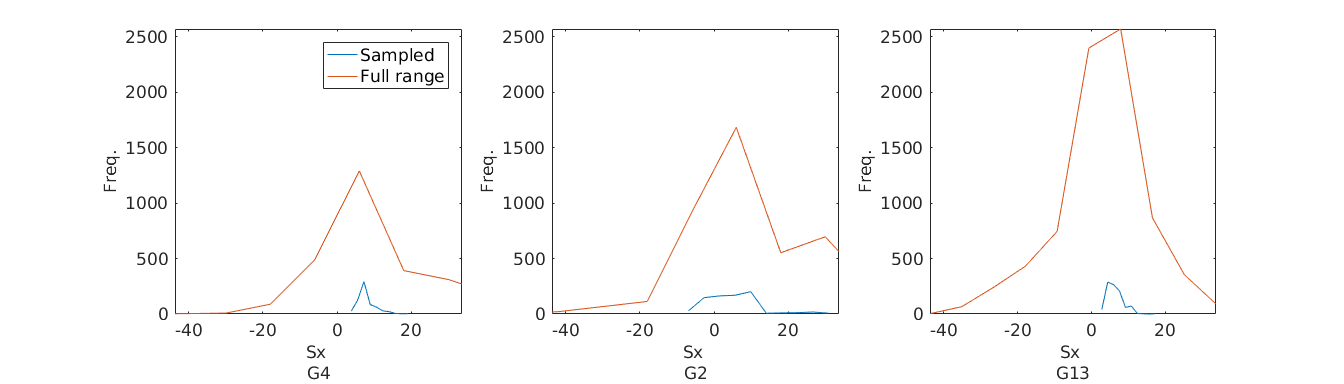
\includegraphics[height = 0.4\textwidth]{SampledRangeTopo_Sx.png}\\
	\caption{Range of $Sx$ sampled as compared to total range of $Sx$ of study glaciers.}
	\label{sampledRange:Sx}
\end{figure}

\end{landscape}


%%%%%%%%%%%%%%%%%%%%%%%%%%%%%%%%%%%%%%%%%%%%%%%%%%
\section{Linear Regressions}

Relating snow accumulation and terrain parameters to better predict accumulation within a basin has been employed for decades \citep[e.g.][]{Woo1978, Molotch2005, McGrath2015}. The most common type of relation between topographic parameters and accumulation is a linear regression, where the observed snow water equivalent (SWE) is related to a linear combination of topographic parameters at each measurement location. 

A linear regression takes the form
\begin{equation}
\vector{y} = \vector{X} \bm{\beta} + \bm{\varepsilon},
\end{equation}
where the matrix $\vector{X}$ contains the set of independent regressors $\vector{x}_i$ used to explain the dependant variable $\vector{y}$ \citep{Davis1986}. The regression coefficients for each regressor is given by $\bm{\beta}$ and the error or noise of the system is given by $\bm{\varepsilon}$. Applied to this study, the matrix of independent regressors ($\vector{X}$) contains the topographic parameters at the sampling locations, the dependant variable $\vector{y}$ contains the observed SWE, and the $\bm{\beta}$ values are determined using a fitting model. While there are many types of fitting models, the ones employed in this study are multiple linear regression (MLR) and Bayesian model averaging (BMA).

Once $\bm{\beta}$ values have been estimated, they can then be used to predict values of the dependant variable in other locations where regressors are known \citep{Davis1986}. Known values of topographic parameters can be multiplied by their respective $\bm{\beta}$ coefficients and added together to obtain the modelled or predicted value of SWE for that DEM grid cell.


\subsection{Multiple Linear Regression}
\label{sec:MLR}

\subsubsection{Background}

Perhaps the most basic and well used method for relating SWE and topographic parameters is a multiple linear regression (MLR) \citep[e.g.][]{Cohen2013}. The best fit line of an MLR is the one described by coefficients that minimize the sum of squares of the vertical deviations of each data point from the line \citep{Davis1986}. Note that if a point falls on the line then the deviation is zero and that the positive and negative deviations from the line do not cancel because the values are first squared and then summed. The residuals are simply the difference between the modelled and observed data. 

To reduce the chance of over fitting the data, two additional methods were applied. The first method was model averaging over all possible models that allow for linear combinations of the chosen topographic parameters. An MLR was estimated for each model (total number of models is $2^n$, where $n$ is the number of topographic parameters) and the Bayesian information criterion (BIC) value was computed for the model according to
\begin{equation}
\textrm{BIC} = -2 \ln L(\hat\theta_k  | y) + k \ln(n),
\end{equation}•
where the values of $\hat \theta_k$, which are the model parameters, maximizes the likelihood function for data $y$ \citep{Burnham2004}. The number of data points is $n$ and the number of regressors is $k$. BIC values are used to assess the relative predictive success of models while penalizing for overfitting of data. While the absolute BIC value is meaningless, models can be selected or averaged using the relative BIC value, with lower values indicating a better model \citep{Burnham2004}. 

In this study, there was no reason to favour any of the models so a weighted average of all models based on their BIC values was conducted. The BIC values for each model ($BIC_i$) were used to determine the normalized weight of each model ($w_i$) relative to the best model (lowest BIC value $BIC_{min}$) according to \citep{Burnham2004}
\begin{equation}
w_i = \frac{e^{-0.5(BIC_i-BIC_{min})}}{\Sigma_{i=1}^R e^{-0.5(BIC_i-BIC_{min})}}.
\label{eq:BIC}
\end{equation}
When parameters were excluded from a model, a coefficient of zero was assigned to that parameter. The sum of the weighted coefficients gave the final $\bm{\beta}$ values.

The second method used to prevent over fitting was to calculate the MLRs within a cross validation framework. This meant that for each model, a randomly selected portion of the data was used to estimate regression coefficients and these were used to predict values that correspond to the remaining data \citep{Kohavi1995}. The root mean squared error (RMSE) between the modelled and observed data was then calculated. This process was done one thousand times and the set of coefficients that resulted in the lowest RMSE were then chosen for that model. 

Together, cross validation allowed for reputable choosing of regression coefficients for each possible model and model averaging with BIC weights allowed for stability of final coefficient values and favouring of simpler models, which would help to identify main topographic drivers of snow accumulation. 

\subsubsection{Methods}
\label{sec:MLRMethods}

A multiple linear regression (MLR) between snow water equivalent (SWE) and all linear combinations of the calculated topographic parameters was completed. This methodology for calculating the MLR also involved using cross validation, where a portion of the data is withheld from the MLR fit and these points are then used to assess the ability of the MLR to predict values. The MLR fit with the best prediction ability is then carried forward. 

The MLR was completed with the following steps (executed using the function 'MLRcalval.m'):
\begin{enumerate}
\item The topographic parameters 

\item The \texttt{topo\_sampled} structure for one glacier as well as the \texttt{SWE} strcture is passed into the function.

\item A set of initializations is completed. This includes 1) creating a logical matrix to choose all linear combination of topographic parameters, 2) selecting the number of runs, 3) creating a matrix of random numbers for selecting data point in the cross validation procedure, 4) initializing matrices, and 5) converting the input structure to a table.

\item For each linear combination of topographic parameters, one thousand runs of a cross validation MLR are then executed. Two-thirds of the total data is randomly selected \citep{Kohavi1995} to use for calculating the regression (using the function \texttt{regress()} which is a basic regression function with fast execution). The MLR equations is used to predict the SWE using the remaining one-quarter of the topographic parameters. The root-mean-squared error (RMSE) between the predicted and observed SWE values is then calculated and the MLR equation with the lowest RMSE is then chosen for that combination of topographic parameters. The function \texttt{fitlm()} is then used to calculate the MLR from the set of data that gave the lowest RMSE. This function is slower but calculates a number of additional values that characterize the fit of the model. One of these values is the Bayesian information criterion (BIC), which allows for model selection among a finite set of models \citep{Burnham2004}. The BIC from the best model for each combination of topographic parameters is saved.

\item A weighted sum of all models found using linear combinations of topographic parameters was then found. The BIC values for each model (BIC$_i$) were used to determine the normalized weight of each model ($w_i$) relative to the best model (lowest BIC value BIC$_{min}$) according to Eq. \ref{eq:BIC}.

\item The percent variance ($var_\%$) explained by each parameter was calculated using the equation $var_\% = \frac{SSr}{SSt}\times 100$, where $SSr$ is the sum of squares of the residual (fitted topographic parameters) and $SSt$ is the total sum of squares (SWE observations). The final coefficients and the percent varience explained by each one can be found in the \texttt{coeffs\_final} table within the function and in the \texttt{mlr} structure when run for all density options and glaciers in the main script 'TopoRegression.m'.

\item The residuals of the fit have also been calculated as a separate variable than can be returned when the function is called. The residual was calculated as the difference between the predicted and observed value. 
\end{enumerate}


\subsubsection{Results}

The coefficients determined using MLR for density Option 8 can be seen in Table \ref{tab:MLRcoeff}. These coefficients were found for standardized values of topographic parameters so their magnitude is indicative of their importance in predicting SWE. The range of percent variance explained by each variable (from all density options) can be seen in Figure \ref{fig:PercentVar_densityOptions}. The fit between modelled SWE and observed SWE for each glacier for density Option 8 can be seen in Figure \ref{fig:MLRfit_opt8} and the fit for all density options in Figure \ref{fig:MLRfit_allLines}. The distribution of residuals in then plotted in Figure \ref{fig:MLRresiduals_all}. A map of the predicted values of SWE over the entire glacier using density option 8 can be seen in Figure \ref{fig:MLRmodelledSWE}.

\begin{wraptable}{R}{10cm}
\centering
\caption{MLR coefficients for topographic regression between measured SWE and standardized topographic parameters that include distance from centreline ($d_C$), elevation ($z$), aspect ($\alpha$),slope ($m$), northness ($N$), profile curvature ($\kappa_P$), tangent curvature ($\kappa_T$), and wind redistribution ($Sx$). SInce parameters are standardizes, the magnitude of the coefficients is representative of their importance in predicting SWE. The root-mean-squared error (RMSE) between modelled SWE using those coefficients and observed SWE is also given.}
\label{tab:MLRcoeff}
\begin{tabular}{cccc}
 & \textbf{Glacier 4} & \textbf{Glacier 2} & \textbf{Glacier 13} \\ \hline
d$_C$ & -0.017 & 0.017 & 0.025 \\
$z$ & 0.001 & 0.118 & 0.052 \\
$\alpha$ & \textless0.001 & -0.006 & \textless0.001 \\
$m$ & -0.018 & -0.002 & -0.007 \\
$N$ & 0.001 & \textless0.001 & 0.015 \\
$\kappa_P$ & 0.001 & \textless0.001 & -0.004 \\
$\kappa_T$ & \textless0.001 & \textless0.001 & -0.002 \\
$Sx$ & 0.001 & 0.008 & \textless0.001 \\
Intercept & 0.629 & 0.264 & 0.242 \\ \hline
RMSE &  &  & 
\end{tabular}
\end{wraptable}

For Glacier 4, the largest coefficients are distance from centreline and slope, which are an order of magnitude larger than the remaining coefficients. Both coefficients are negative, which indicates less snow along the margins of the glacier and less on steeper slopes. These coefficients account for the largest percentage of variance explained, although this percentage is very small ($<2$\% each). The map of predicted SWE for the entire glacier closely resembles the distribution of distance from centreline (Figure \ref{map:centreD}), which also shows its dependence on this parameter. Overall, the modelled winter balance for Glacier 4 is very poorly explained by the topographic parameters, which results in no correlation between modelled and observed SWE (R$^2=0.04$). The modelled values of SWE are largely determined by the intercept value. RMSE???

For Glacier 2, the largest coefficient (by an order of magnitude) is elevation. This coefficient is positive, which means that SWE will increase with elevation. Elevation explains the largest amount of variance (52\%) and this is consistent for all density options. The map of modelled SWE shows this strong dependence on elevation since the values closely resemble the elevation map (Figure \ref{map:elev}). Overall, the modelled winter balance is moderately good estimation of observed SWE (R$^2=0.57$) although it tends to underestimate the amount of accumulation. 

For Glacier 13, the largest coefficient is elevation with distance from centreline and ``northness'' also of the same order of magnitude. All three coefficients are positive, which means that cell at higher elevation, closer to the margins, and more north facing had higher amounts of SWE. Elevation explains the majority of the variance (24\%), while distance from centreline and ``northness'' explain far less ($<$3\% each). The map of modelled SWE displays an increase with elevation, although it is not strong considering the large range of elevation on this glacier. Overall, the MLR modelled winter balance is poorly related to observed SWE (R$^2=0.3$) and tends to underestimate the amount of accumulation.

Qualitatively, there is little variation in the fit between modelled and observed winter balance between the various density options for all glaciers and the residuals display a similar distribution between the density options.The percent variance explained by each parameter also varies little between different density options. 


\begin{landscape}
\begin{figure}
	\centering
	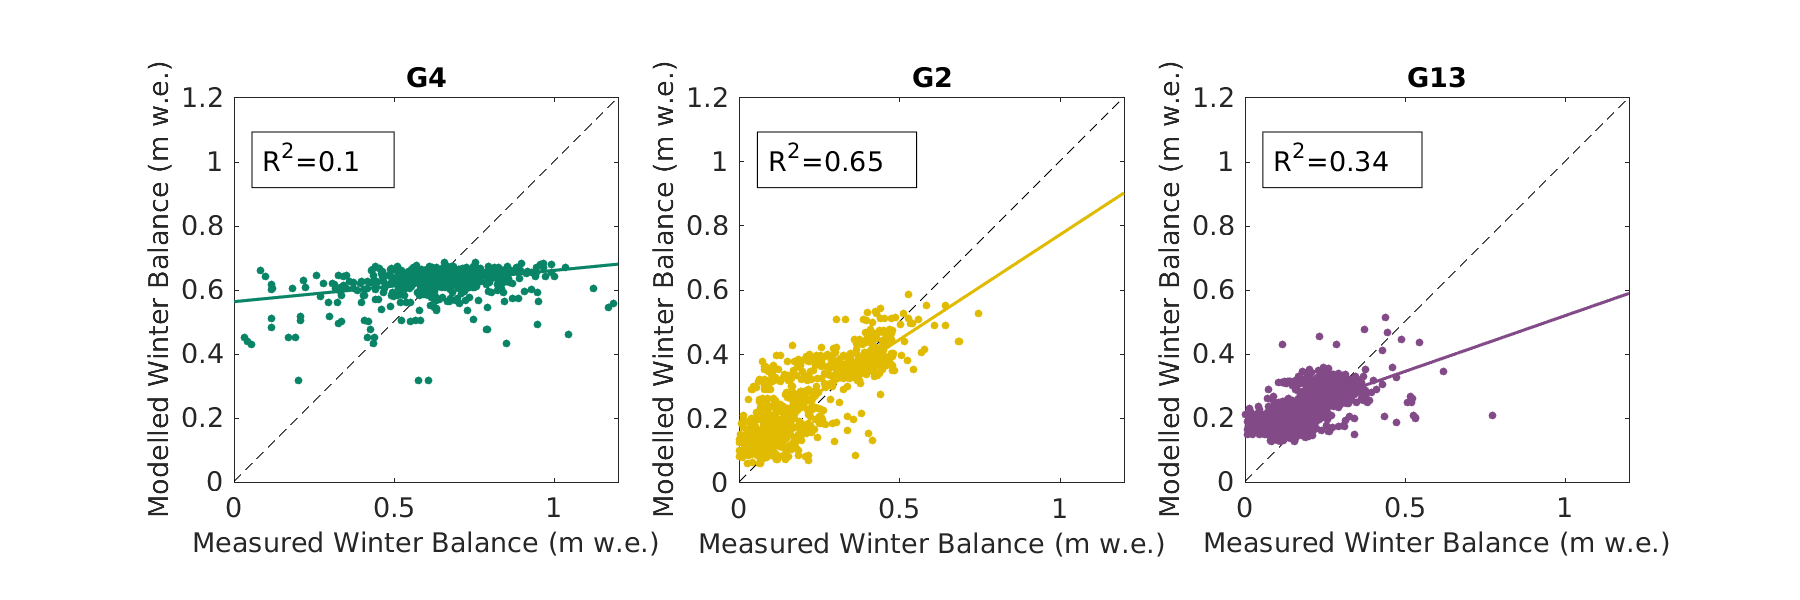
\includegraphics[height = 0.4\textwidth]{MLRfit_opt8.png}\\
	\caption{Comparison of predicted (MLR) and observed (original) snow water equivalent (SWE) for three study glaciers. The SWE values were calculated inverse distance weighted snowpit densities (Option 8).}
	\label{fig:MLRfit_opt8}
\end{figure}

\pagebreak

\begin{figure}
	\centering
	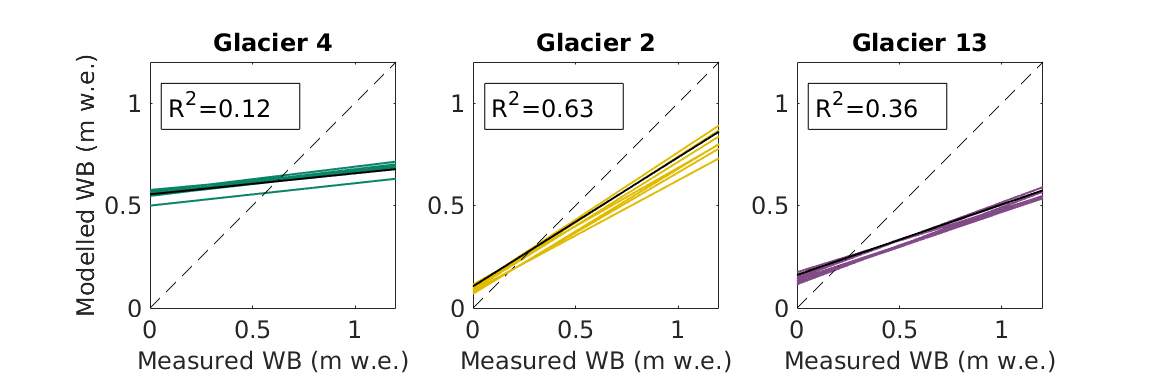
\includegraphics[height = 0.4\textwidth]{MLRfit_allLines.png}\\
	\caption{Plot of all linear fits between modelled and observed SWE using eight options for calculating density. Mean R$^2$ value is shown for each sub-plot and a reference 1:1 line is also provided. See Figure \ref{fig:MLRfit_opt8} for a plot of the data. }
	\label{fig:MLRfit_allLines}
\end{figure}

\begin{figure}
	\centering
	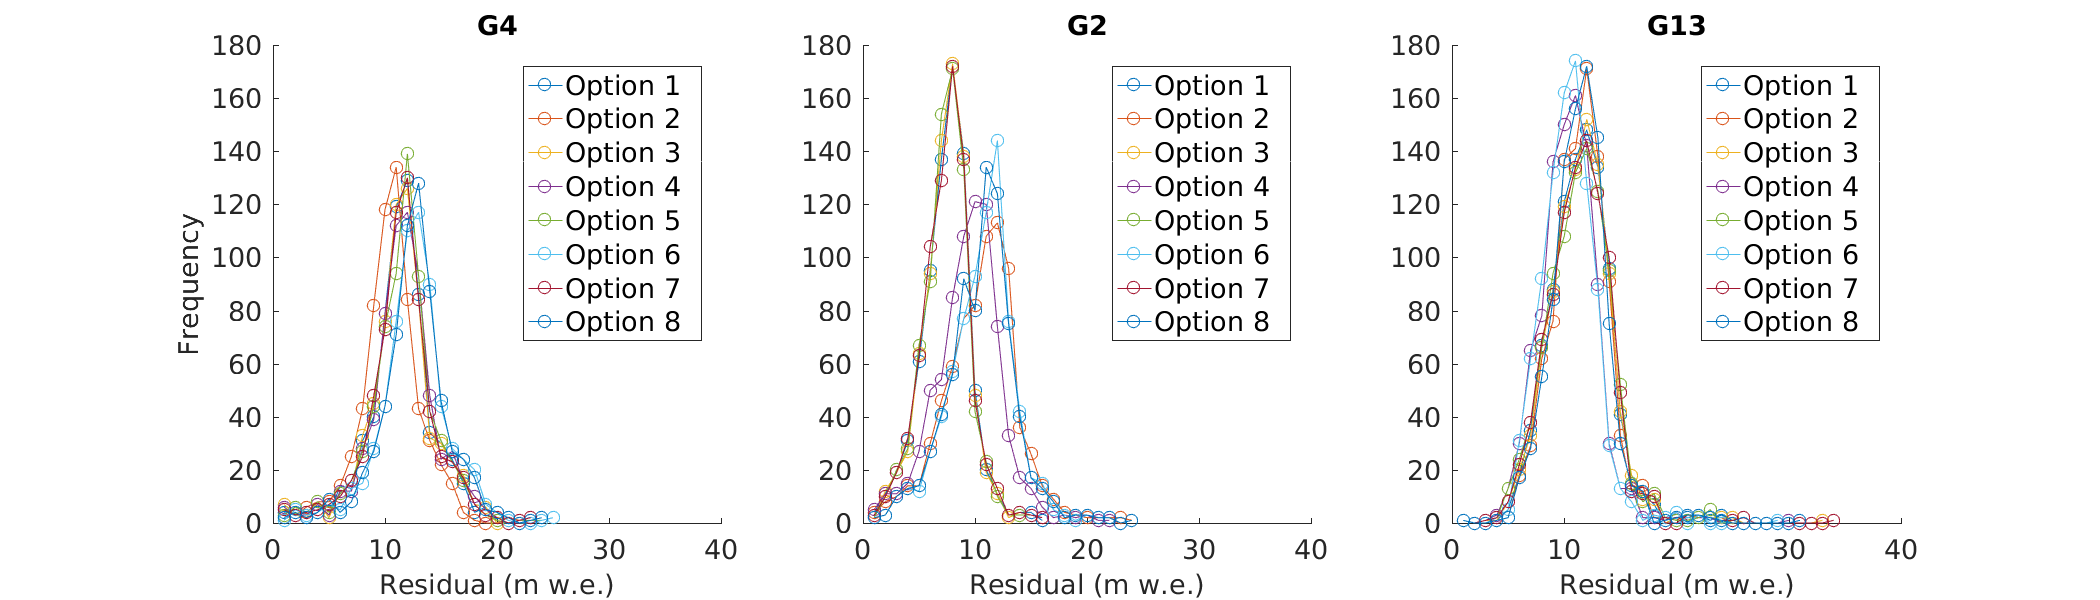
\includegraphics[height = 0.4\textwidth]{MLRresiduals_all.png}\\
	\caption{Residuals of SWE predicted using MLR for all options of estimating density.}
	\label{fig:MLRresiduals_all}
\end{figure}

\end{landscape}
 
\begin{figure}[H]
	\centering
	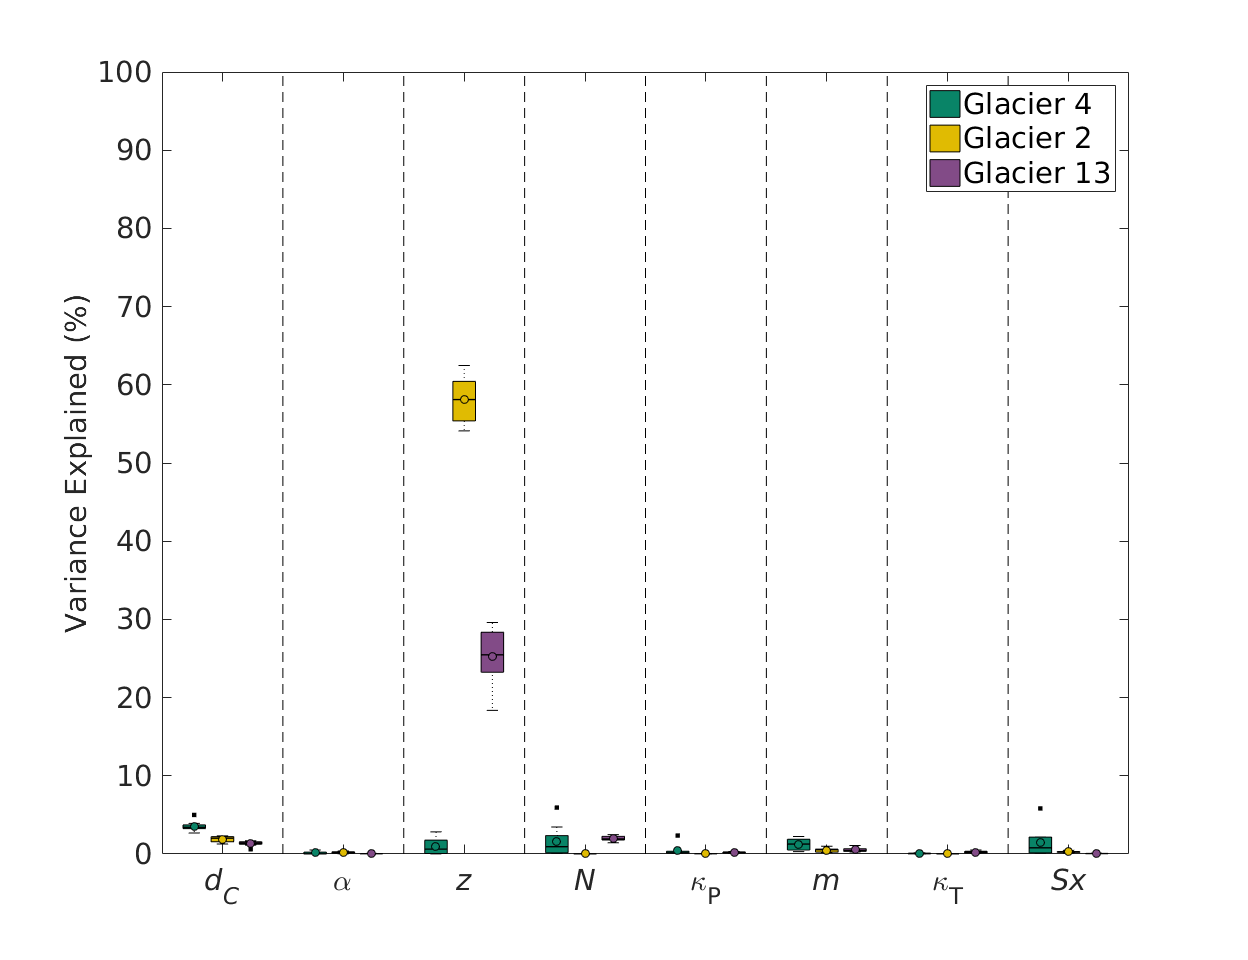
\includegraphics[width =1.1 \textwidth]{Coeffs_DensityOpts.png}\\
	\caption{Boxplot showing the range of percent variance explained by each topographic parameter for each option of estimating snow water equivalent (SWE). Topographic parameters include aspect ($\alpha$), elevation ($z$), northness ($N$), profile curvature ($\kappa_P$), slope ($m$), tangent curvature ($\kappa_T$), wind redistribution ($Sx$) and distance from centreline ($d_C$).}
	\label{fig:MLRPercentVar_densityOptions}
\end{figure} 

%\begin{landscape}
%\begin{figure}
%	\centering
%	\includegraphics[height = 0.9\textwidth]{MLRmap_Modelled_Observed.png}
%	\caption{Modelled SWE using coefficients determined using MLR and density interpolated with inverse-distance weighting from snowpits. Observed SWE values are overlain on the maps.}
%	\label{fig:MLRmodelledSWE}
%\end{figure}
%\end{landscape}


%%%%%%%%%%%%%%%%%%%%%%%%%%%%%%%%%%%%%%%%%%%%%%%%%%
\subsection{Bayesian Model Averaging}
\label{sec:BMS}

\subsubsection{Background}

\begin{wrapfigure}{L}{0.6\textwidth}
	\centering
	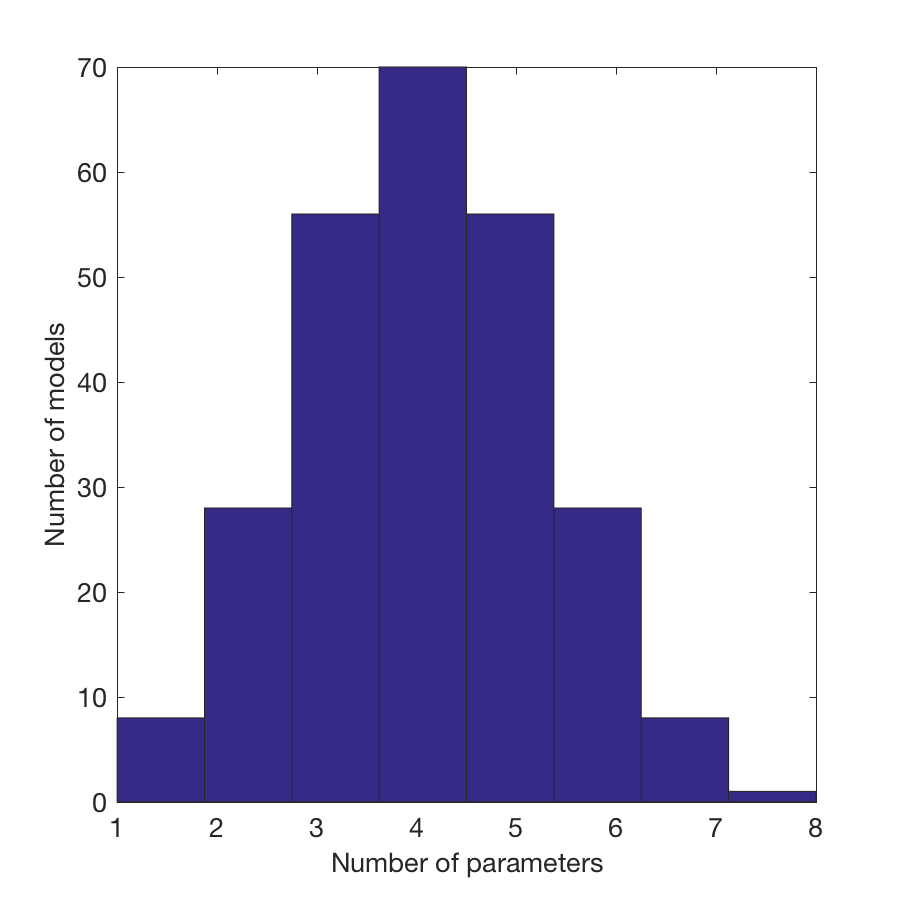
\includegraphics[width = 0.6\textwidth]{DistributionOfNumParams_topoRegress.png}\\
	\caption{Uniform model prior for eight topographic regressors used in BMA.}
	\label{fig:uni_model_prior}
\end{wrapfigure}

Bayesian model averaging (BMA) is a method of estimating all possible linear combinations of predictor variables and then averaging over all models \citep{Raftery1997, Wasserman2000, Raftery2005}.  This method is based on Bayesian principals where we wish to determine the probability of an outcome based on an initial ``guess'' as well as the data provided. Given that the predictive outcome has a probability distribution of $x$ given $y$, written as $P(x|y)$, we use Bayes' rule to to write this as
\begin{equation}
P(x|y) = \frac{P(y|x)P(x)}{P(y)}.
\end{equation}•
$P(x|y)$ is often called the posterior model probability (PMP). The quantity $P(y|x)$ is the likelihood function, which determines unknown parameters from a known outcome (i.e. observed data). The term $P(x)$ is an observer determined prior probability distribution (typically just called a \textit{prior}) and it reflects the prior knowledge of the system \citep{Raftery1997}. Choosing an appropriate prior is one of the most challenge components of Bayesian probability theory \citep{Wasserman2000}. The$P(y)$ term can be obtained by integrating $P(y|x)P(x)$ over all $x$ and is thus a constant for all models that is typically discarded \citep{Wasserman2000}. 

Together then, the posterior model probability is a function of both the model prior, specified by the researcher, as well as the distribution of the observed data --- it is the transformation of the prior as a result of considering collected data \citep{Wasserman2000}. This can be loosely expressed as
\begin{equation}
\textrm{posterior} \propto \textrm{prior} \times \textrm{likelihood}
\end{equation}
If the prior is uninformative then the posterior will be strongly influenced by the data \citep{Wasserman2000}. An informative prior will result in a posterior that is a mix of the prior and the data as as the prior becomes more informative, the amount of data needed to transform the distribution increases. If there is a large amount of data then the prior will have little effect on the posterior. The final value of the desired output is often reported as the posterior distribution mean or the value that maximizes the log-likelihood. 

Within BMA, Bayes' theorem is used to find the posterior model probability and this is used as a weight when averaging over all models \citep{Wasserman2000}. The model weighted posterior distribution for the coefficients $\beta$ of $k$ number of models after renormalization is given by 
\begin{equation}
P(\beta\ | y,X) = \sum\limits_{i=1}^{2^k} P(M_i | X,y)P(\beta | M_i , y, X),
\end{equation}
where the responding variable is given by $y$ and the matrix of variables is given by $X$ \citep{Raftery1997}. Here, the model prior is $P(M_i | X,y)$ and the likelihood for the $\beta$ coefficient is $P(\beta | M_i , y, X)$.

There are a number of different priors to describe model size distribution that have been applied in BMA. A commonly used prior is the `uniform' prior, which assumes a normal model distribution with a total of $2^n$ models, where $n$ is the number of regressors \citep{Wasserman2000}.  This model prior states that the observer has no knowledge of the system and all models are equally likely. The uniform prior has a prior model probability of the form $P(M_i)=2^{-n}$, as shown in Figure \ref{fig:uni_model_prior}, which is symmetric about the mean $n/2$ \citep{Zeugner2015}. This prior inherently favours models of an intermediate size. 

Other types of priors include those that are skewed to favour smaller models, ones with equal probability for all model sizes, and ones with varying probability for individual regressors. In this project, a uniform prior was chosen because there was no knowledge of what the model distribution would look like and to match the distribution of models sizes in the MLR analysis. This is commonly done in BMA \citep{Wasserman2000}.

With a small number of regressors, the posterior of all possible models can be determined. As the number of regressors increases, this computation becomes increasingly expensive since the total number of models is $2^n$. To overcome this, BMA can use Markov chain Monte Carlo (MCMC) model composition to directly approximate the posterior distribution \citep{Wasserman2000}. In our study, there are eight regressors, resulting in $2^8 = 256$models. It is possible to visit all models and to obtain an exact solution so an MCMC model composition was not employed. 

BMA allows for the calculation of a metric called the posterior inclusion probability (PIP), which is used to evaluate the importance of a regressor in explaining the observed data. PIP is the sum of all posterior model probabilities (PMP) where the variable was included in the mode \citep{Zeugner2015}l. A higher PIP indicates that the regressor is more important in the regression.  

\subsubsection{Methods}

The BMA process was implemented in R, using the Bayesian model statistics (BMS) package developed by \cite{Zeugner2015}. The function \texttt{BMS\_R()} computes the $\beta$ coefficients for all topographic parameters for all study glaciers as well as the percent variance explained by each parameter suing the following steps:
\begin{enumerate}
\item The SWE observations and associated topographic parameters are called in the function.
\item A portion of the data ($2/3$ as suggested by \cite{Kohavi1995}) is randomly chosen as the calibration set and saved as a .mat file. 
\item The R script is called through the terminal
	\begin{enumerate}
		\item The R script imports the .mat file with SWE and topographic parameter values. It then creates a data 				frame with the SWE values as the first column and the topographic parameters as the remaining 					columns. 
		\item The BMS package is used to complete BMA for the imported values. A uniform model prior was chosen. 				The mean coefficient value, coefficient standard deviation, PIP, and the posterior probability of a positive 			coefficient (how probable it is for the sign of the coefficient to be positive) were computed.
		\item The coefficients are saved as a .mat file.
	\end{enumerate}•
\item Values calculated in R are loaded into Matlab and a data table is created with the coefficients.
\item The remaining portion of the topographic parameter values ($1/4$) are then used to calculate a modelled value of 		SWE at those locations. These are compared to the observed SWE values and a RMSE value is determined.
\item The above step are completed 1000 times and the coefficients associated with the lowest RMSE are chosen.
\item Percent variance explained by each parameter is the calculated in the same way as for the MLR (see Section 			\ref{sec:MLRMethods}). 
\item The final table of values includes the coefficients and percent variance explained for all topographic parameters associated with the lowest RMSE. It also includes the intercept and the actual RMSE value. This table is returned from the function.
\item The residuals of the best BMA fit are also calculated and can be return from the function.  
\end{enumerate}•



\subsubsection{Results}

The coefficients determined using BMA for density Option 8 can be seen in Table \ref{tab:BMScoeff}. These coefficients were found for standardized values of topographic parameters so their magnitude is indicative of their importance in predicting SWE. The range of percent variance explained by each variable (from all density options) can be seen in Figure \ref{fig:BMSPercentVar_densityOptions}. The fit between modelled SWE and observed SWE for each glacier for density option 8 can be seen in Figure \ref{fig:BMSfit_opt8} and the fit for all density options in Figure \ref{fig:BMSfit_allLines}. The distribution of residuals in then plotted in Figure \ref{fig:BMSresiduals_all}. A map of the predicted values of SWE over the entire glacier using density option 8 can be seen in Figure \ref{fig:BMSmodelledSWE}.

\begin{wraptable}{R}{10cm}
\centering
\caption{BMS coefficients for topographic regression between measured SWE and standardized topographic parameters that include distance from centreline ($d_C$), elevation ($z$), aspect ($\alpha$),slope ($m$), northness ($N$), profile curvature ($\kappa_P$), tangent curvature ($\kappa_T$), and wind redistribution ($Sx$). SInce parameters are standardizes, the magnitude of the coefficients is representative of their importance in predicting SWE. The root-mean-squared error (RMSE) between modelled SWE using those coefficients and observed SWE is also given.}
\label{tab:BMScoeff}
\begin{tabular}{cccc}
 & \textbf{Glacier 4} & \textbf{Glacier 2} & \textbf{Glacier 13} \\ \hline
d$_C$ & -0.028 & 0.021 & 0.015 \\
$z$ &  \textless0.001 & 0.118 & 0.051 \\
$\alpha$ & -0.001 & -0.001 & 0.001 \\
$m$ & -0.014 & 0.002 & -0.004 \\
$N$ &  \textless0.001 & \textless0.001 & 0.014 \\
$\kappa_P$ & 0.001 & \textless0.001 & -0.001 \\
$\kappa_T$ & \textless0.001 & \textless0.001 & -0.002 \\
$Sx$ & 0.002 & \textless0.001 & \textless0.001 \\
Intercept & 0.623 & 0.266 & 0.242 \\ \hline
RMSE &  &  & 
\end{tabular}
\end{wraptable}

For Glacier 4, the largest coefficients are distance from centreline and slope, which are an order of magnitude larger than the remaining coefficients. Both coefficients are negative, which indicates less snow along the margins of the glacier and less on steeper slopes. These coefficients account for the largest percentage of variance explained, although this percentage is very small ($<3$\% each). The map of predicted SWE for the entire glacier closely resembles the distribution of distance from centreline (Figure \ref{map:centreD}), which also shows its dependence on this parameter. Overall, the modelled winter balance for Glacier 4 is very poorly explained by the topographic parameters, which results in no correlation between modelled and observed SWE (R$^2=0.05$). The modelled values of SWE are largely determined by the intercept value. RMSE???

For Glacier 2, the largest coefficient (by an order of magnitude) is elevation. This coefficient is positive, which means that SWE will increase with elevation. Elevation explains the largest amount of variance (52\%) and this is consistent for all density options. The map of modelled SWE shows this strong dependence on elevation since the values closely resemble the elevation map (Figure \ref{map:elev}). The second largest coefficient is distance from centreline, which accounts for 2\% of the variance. Overall, the modelled winter balance is a good estimation of observed SWE (R$^2=0.62$) although it tends to underestimate the amount of accumulation. 

For Glacier 13, the largest coefficient is elevation with distance from centreline and ``northness'' also of the same order of magnitude. All three coefficients are positive, which means that cells at higher elevation, closer to the margins, and more north facing had higher amounts of SWE. Elevation explains the majority of the variance (23\%), while distance from centreline and ``northness'' explain far less ($<$2\% each). The map of modelled SWE displays an increase with elevation, although it is not strong, especially considering the large range of elevation on this glacier. Overall, the MLR modelled winter balance is poorly related to observed SWE (R$^2=0.34$) and tends to underestimate the amount of accumulation.

Qualitatively, there is little variation in the fit between modelled and observed winter balance between the various density options for all glaciers and the residuals display a similar distribution between the density options.The percent variance explained by each parameter also varies little between different density options. 

\begin{landscape}
\begin{figure}
	\centering
	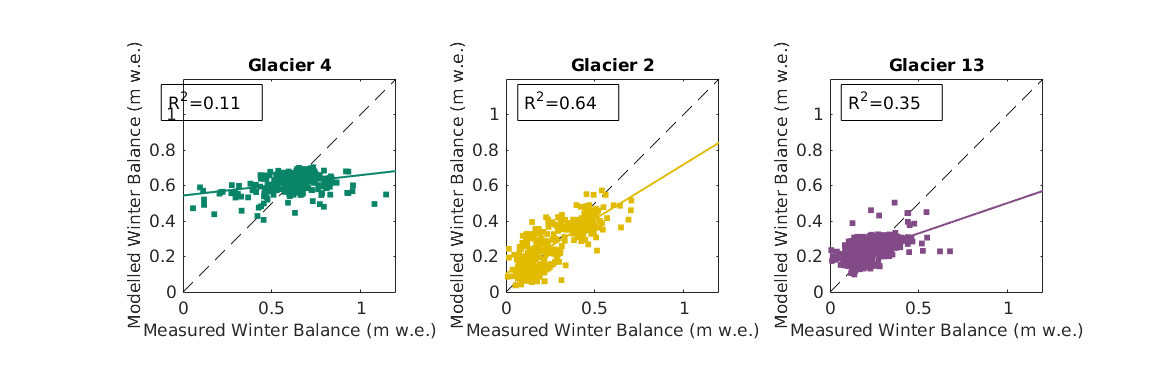
\includegraphics[height = 0.5\textwidth]{BMSfit_opt8.png}\\
	\caption{Comparison of predicted (BMA) and observed (original) snow water equivalent (SWE) for three study glaciers. The SWE values were calculated inverse distance weighted snowpit densities (Option 8).}
	\label{fig:BMSfit_opt8}
\end{figure}

\pagebreak

\begin{figure}
	\centering
	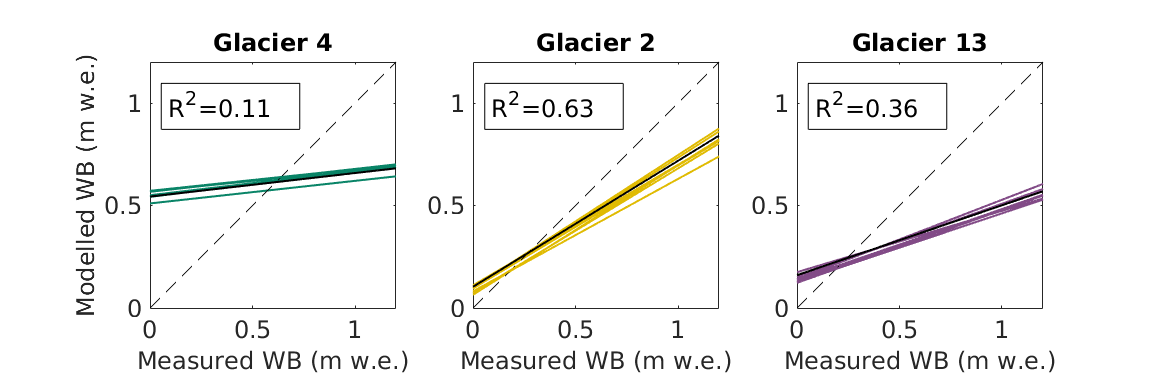
\includegraphics[height = 0.4\textwidth]{BMSfit_allLines.png}\\
	\caption{Plot of all linear fits between modelled (BMA) and observed SWE using eight options for calculating density. Mean R$^2$ value is shown for each sub-plot and a reference 1:1 line is also provided. See Figure \ref{fig:BMSfit_opt8} for a plot of the data. }
	\label{fig:BMSfit_allLines}
\end{figure}

\begin{figure}
	\centering
	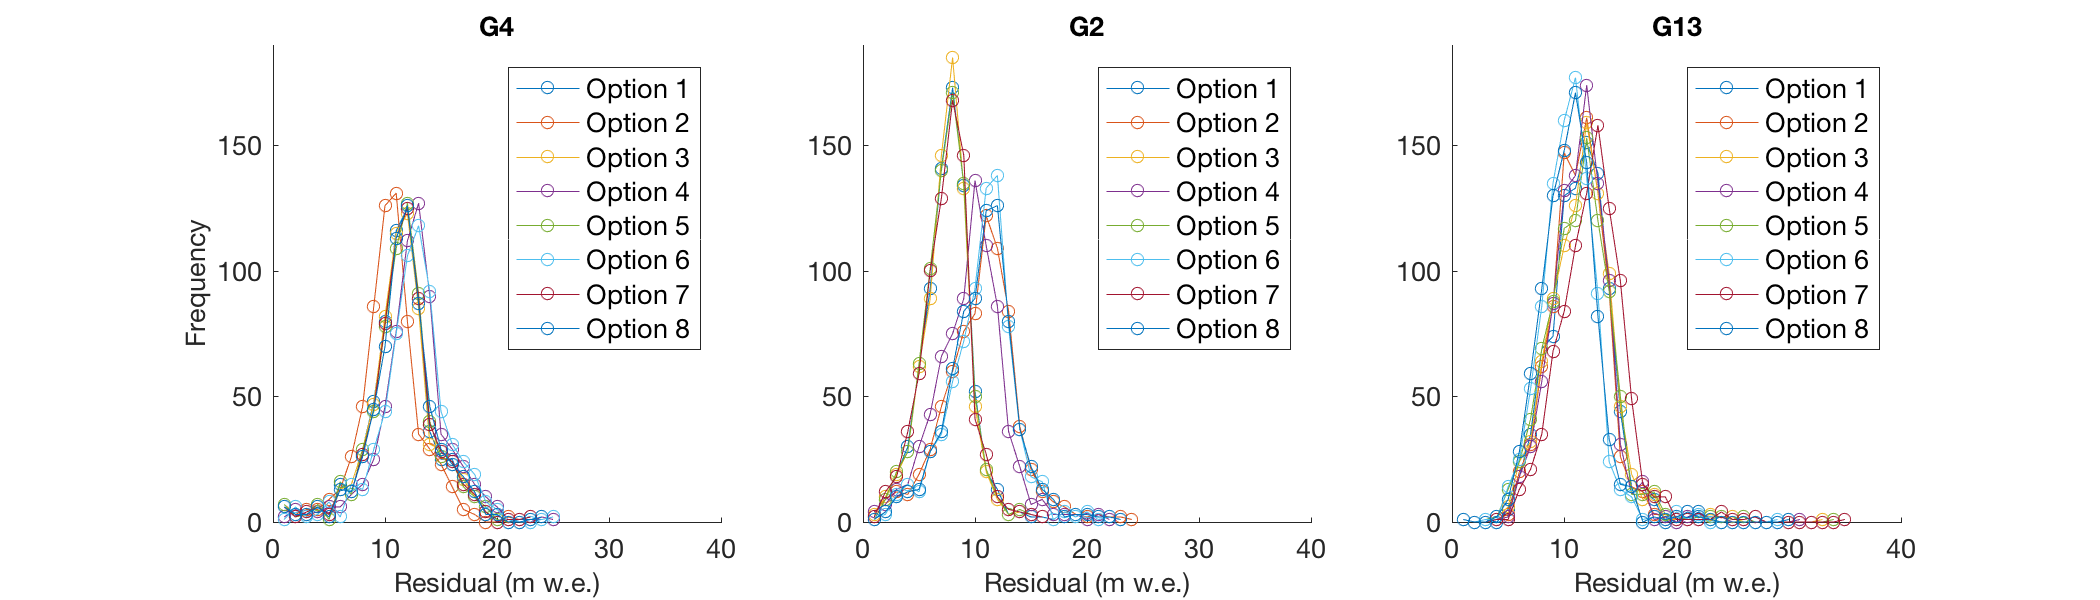
\includegraphics[height = 0.4\textwidth]{BMSresiduals_all.png}\\
	\caption{Residuals of SWE predicted using BMA for all options of estimating density.}
	\label{fig:BMSresiduals_all}
\end{figure}

\end{landscape}
 
\begin{figure}[H]
	\centering
	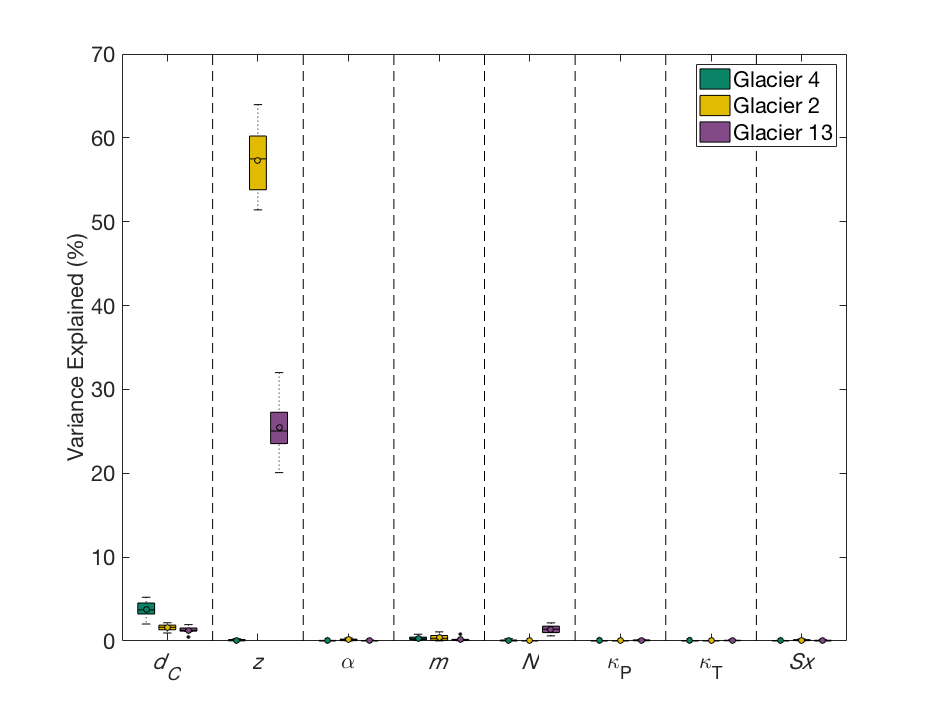
\includegraphics[width =1.1 \textwidth]{BMSCoeffs_DensityOpts.png}\\
	\caption{Boxplot showing the range of percent variance explained by each topographic parameter as calculated using BMA for each option of estimating snow water equivalent (SWE). Topographic parameters include aspect ($\alpha$), elevation ($z$), northness ($N$), profile curvature ($\kappa_P$), slope ($m$), tangent curvature ($\kappa_T$), wind redistribution ($Sx$) and distance from centreline ($d_C$).}
	\label{fig:BMSPercentVar_densityOptions}
\end{figure} 

%\begin{landscape}
%\begin{figure}
%	\centering
%	\includegraphics[height = 0.9\textwidth]{BMSmap_Modelled_Observed.png}
%	\caption{Modelled SWE using coefficients determined using BMA and density interpolated with inverse-distance weighting from snowpits. Observed SWE values are overlain on the maps.}
%	\label{fig:BMSmodelledSWE}
%\end{figure}
%\end{landscape}


%%%%%%%%%%%%%%%%%%%%%%%%%%%%%%%%%%%%%%%%%%%%%%%%%%
\subsection{MLR and BMS comparison}


\begin{figure}[H]
	\centering
	\includegraphics[width =1.1 \textwidth]{Coeff_Compare.png}\\
	\caption{Boxplot showing the range of value for each topographic parameter from both MLR and BMA analysis. Topographic parameters include aspect ($\alpha$), elevation ($z$), northness ($N$), profile curvature ($\kappa_P$), slope ($m$), tangent curvature ($\kappa_T$), wind redistribution ($Sx$) and distance from centreline ($d_C$).}
	\label{fig:allCeoffs_boxplot}
\end{figure} 

\begin{landscape}
\begin{figure}
	\centering
	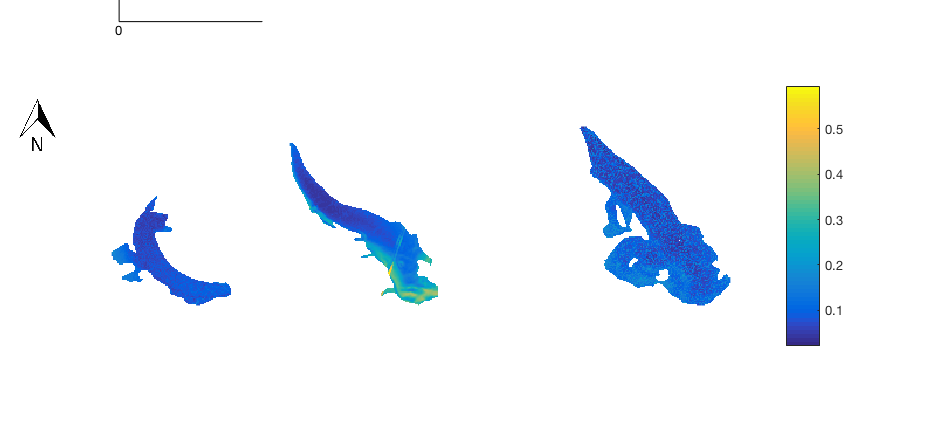
\includegraphics[height = 0.5\textwidth]{SWEdifferenceMap.png}\\
	\caption{Map of the difference between maximum and minimum SWE values for each DEM cell between all density options and from both MLR and BMA.}
	\label{fig:SWEdiffMap}
\end{figure}
\end{landscape}
	
%%%%%%%%
\pagebreak
\bibliography{/home/glaciology1/Documents/MastersDocuments/MastersLit}
\bibliographystyle{igs}

\end{document}